% COLORS
% The following standard colors are defined: wasp_text, wasppink, waspgrey, waspblue

\documentclass[a0paper,portrait]{baposter}
\usepackage{lipsum}  
\usepackage{relsize}	% For \smaller
\usepackage{url}	% For \url
\usepackage{epstopdf}	% Included EPS files automatically converted to PDF to include with pdflatex
\usepackage[utf8]{inputenc} 
\usepackage{multirow}
\usepackage{booktabs}
\usepackage[labelfont=bf]{caption}
\usepackage{enumitem}
\usepackage{tcolorbox}
\usepackage{mathtools}

% PATHS
\graphicspath{{images/content/}{images/template/}}

% FONTS AND COLORS
\renewcommand{\familydefault}{\sfdefault}
\newcommand{\mytitlefont}{\fontfamily{\familydefault}\selectfont }
\newcommand{\mytextfont}{\fontfamily{\familydefault}\selectfont }
% Comment the four lines below to skip WASP fonts
%\usepackage{MinionPro}
%\usepackage{MyriadPro}
\renewcommand{\mytitlefont}{\fontfamily{MyriadPro-LF}\selectfont }
\renewcommand{\mytextfont}{\fontfamily{MinionPro-LF}\selectfont }

\definecolor{wasppink}{RGB}{203,166,169} 
\definecolor{waspgrey}{RGB}{88,89,91}
\definecolor{waspblack}{RGB}{0,0,0}
\definecolor{waspblue}{RGB}{26,141,173}
\definecolor{darkgreen}{rgb}{0,0.6,0}

\definecolor{wasp_text}{RGB}{66,80,82}
\colorlet{wasp_banner_light}{waspblue}
\colorlet{wasp_banner_grey}{waspgrey}
\colorlet{wasp_banner_dark}{waspblack}

% LIST SETTINGS
\setlist{itemsep=.1em, leftmargin=1em}

% COMMANDS
\newcommand\thetitle{}\renewcommand\title[1]{\renewcommand\thetitle{#1}}
\newcommand\theauthor{}\renewcommand\author[1]{\renewcommand\theauthor{#1}}
\newcommand\thedepinfo{}\newcommand\depinfo[1]{\renewcommand\thedepinfo{#1}}
\newcommand\thesupervisors{}\newcommand\supervisors[1]{\renewcommand\thesupervisors{#1}}
\newcommand\theuniversitylogo{}\newcommand\universitylogo[1]{\renewcommand\theuniversitylogo{#1}}
\newcommand\thecompanylogo{}\newcommand\companylogo[1]{\renewcommand\thecompanylogo{#1}}


%%%%%%%%%%%%%%%%%%%%%%%%%%%%%%%%%%%%%%%%%%%%%%%%%%%%%%%%%%%%%%%%%%%%%%%%%%%%%%%
%%% Document Start %%%%%%%%%%%%%%%%%%%%%%%%%%%%%%%%%%%%%%%%%%%%%%%%%%%%%%%%%%%%
%%%%%%%%%%%%%%%%%%%%%%%%%%%%%%%%%%%%%%%%%%%%%%%%%%%%%%%%%%%%%%%%%%%%%%%%%%%%%%%

% Text to the left
\title{GPU parallelization of particle deposition in human lung airways}
\author{Lokesh Mohanty, Thivin Anandh, Sashikumaar Ganesan}
\depinfo{STARS Lab}
% \supervisors{Prof. Sashikumaar Ganesan}

% Logos on the right. Put the images in images/template/
\universitylogo{
\includegraphics[width=0.8\textwidth]{iisc}}
\companylogo{
\includegraphics[width=0.8\textwidth]{cds}}


\begin{document}

%%% General Poster Settings %%%%%%%%%%%%%%%%%%%%%%%%%%%%%%%%%%%%%%%%%%%%%%%%%%%
%%%%%% Eye Catcher, Title, Authors and University Images %%%%%%%%%%%%%%%%%%%%%%
\begin{poster}{
 % Show grid to help with alignment
 grid=false,
 % eyecatcher=false,
 % Column spacing
 colspacing=1em,
 columns=2,
 boxpadding=.5cm,
 % Color style
 headerColorOne=wasp_banner_light,
 borderColor=wasp_banner_light,
 headerFontColor=cyan!10!white,
 % Format of textbox
 textborder=faded,
 % Format of text header
 headerborder=open,
 headershape=roundedright,
 headershade=plain,
 background=none,
 % bgColorOne=cyan!10!white,
 headerheight=0.12\textheight}
%%% Eye Cacther %%%%%%%%%%%%%%%%%%%%%%%%%%%%%%%%%%%%%%%%%%%%%%%%%%%%%%%%%%%%%%%
{
	Eye Catcher, empty if option eyecatcher=false - unused
}
%%%% Title %%%%%%%%%%%%%%%%%%%%%%%%%%%%%%%%%%%%%%%%%%%%%%%%%%%%%%%%%%%%%%%%%%%%%
{
	\textcolor{wasp_text}{\mytitlefont \huge \thetitle}
}
%%% Authors %%%%%%%%%%%%%%%%%%%%%%%%%%%%%%%%%%%%%%%%%%%%%%%%%%%%%%%%%%%%%%%%%%%
{
  \vspace{0.5em}
  \textcolor{wasp_text}{\Large \theauthor\\
	\large \thedepinfo\\
	}
}
%%% Logo %%%%%%%%%%%%%%%%%%%%%%%%%%%%%%%%%%%%%%%%%%%%%%%%%%%%%%%%%%%%%%%%%%%%%%
{
  \begin{minipage}{8cm}
   \centering
  \begin{minipage}{4cm}
    \centering
		  \thecompanylogo
  \end{minipage}
  \begin{minipage}{4cm}
    \centering
	    \theuniversitylogo
  \end{minipage}
  \end{minipage}
}

%%%%%%%%%%%%%%%%%%%%%%%%%%%%%%%%%%%%%%%%%%%%%%%%%%%%%%%%%%%%%%%%%%%%%%%%%%%%%%
%%% Now define the boxes that make up the poster
%%%---------------------------------------------------------------------------
%%% Each box has a name and can be placed absolutely or relatively.
%%% The only inconvenience is that you can only specify a relative position 
%%% towards an already declared box. So if you have a box attached to the 
%%% bottom, one to the top and a third one which should be inbetween, you 
%%% have to specify the top and bottom boxes before you specify the middle 
%%% box.
%%%%%%%%%%%%%%%%%%%%%%%%%%%%%%%%%%%%%%%%%%%%%%%%%%%%%%%%%%%%%%%%%%%%%%%%%%%%%%

%%%%%%%%%%%%%%%%%%%%%%%%%%%%%%%%%%%%%%%%%%%%%%%%%%%%%%%%%%%%%%%%%%%%%%%%%%%%%%
  \headerbox{\mytitlefont Motivation \& Research Goals}{name=description,column=0,row=0,span=2}{
  \mytextfont
%%%%%%%%%%%%%%%%%%%%%%%%%%%%%%%%%%%%%%%%%%%%%%%%%%%%%%%%%%%%%%%%%%%%%%%%%%%%%%
  % Put the motivation behind and goals of the research here
\large
Modeling particle deposition in human air pathways is important for understanding regional particle deposition which is crucial for targeted drug delivery. Studies have shown potential health risks associated with ultrafine particles deposited in lungs. Traditional techniques of in vivo and in vitro face significant challenges. And the commonly used Lagrangian approach is computationally intensive as it involves the tracking and interpolating of millions of particles at each time step. Due to the intricate nature of finite element method data structures, parallelizing the particle deposition on GPUs poses challenges.

}

%%%%%%%%%%%%%%%%%%%%%%%%%%%%%%%%%%%%%%%%%%%%%%%%%%%%%%%%%%%%%%%%%%%%%%%%%%%%%%
  \headerbox{\mytitlefont Methodology}{name=motivation,column=0,row=0,span=1, below=description}{
%%%%%%%%%%%%%%%%%%%%%%%%%%%%%%%%%%%%%%%%%%%%%%%%%%%%%%%%%%%%%%%%%%%%%%%%%%%%%%
  \mytextfont
  % The methods that you use goes here

Using ParMooN\textsuperscript{[1]}, an in-house FEM package, we solve the time dependent Navier-Stokes equation using variational multi-scale method. And using its results, the particles are simulated by a Lagrangian approach\textsuperscript{[2]}. The equations of motion for the particles are given by

\begin{alignat*}{2}
     m_p\frac{d\mathbf{u}_p}{dt} =& \frac{3}{4}\frac{\rho_f}{\rho_p}\frac{m_p}{d_p}\frac{C_D}{C_C}\left|\mathbf{u}_f - \mathbf{u}_p\right|\left(\mathbf{u}_f - \mathbf{u}_p\right)  \\
     &+ m_p\mathbf{g}\frac{\rho_p - \rho_f}{\rho_p} + \mathbf{F}_B
\end{alignat*}

Here $\mathbf{u}_p$, $\mathbf{u}_f$, $\rho_p$, $\rho_f$,  represents the particle velocity, fluid velocity, particle density and fluid density respectively. The terms in the right hand side are drag force, gravitational force and Brownian force respectively.

\begin{itemize}
\item The above equation is used to update the particle's current position at every time-step
\item Based on the current position, the current cell is determined using a zonal-based search
\item If the particle is outside the domain, based on the previous cell and current position, the deposition location is computed
\end{itemize}

\vspace{0.3cm}
\begin{center}
  \vspace{-0.4cm}
  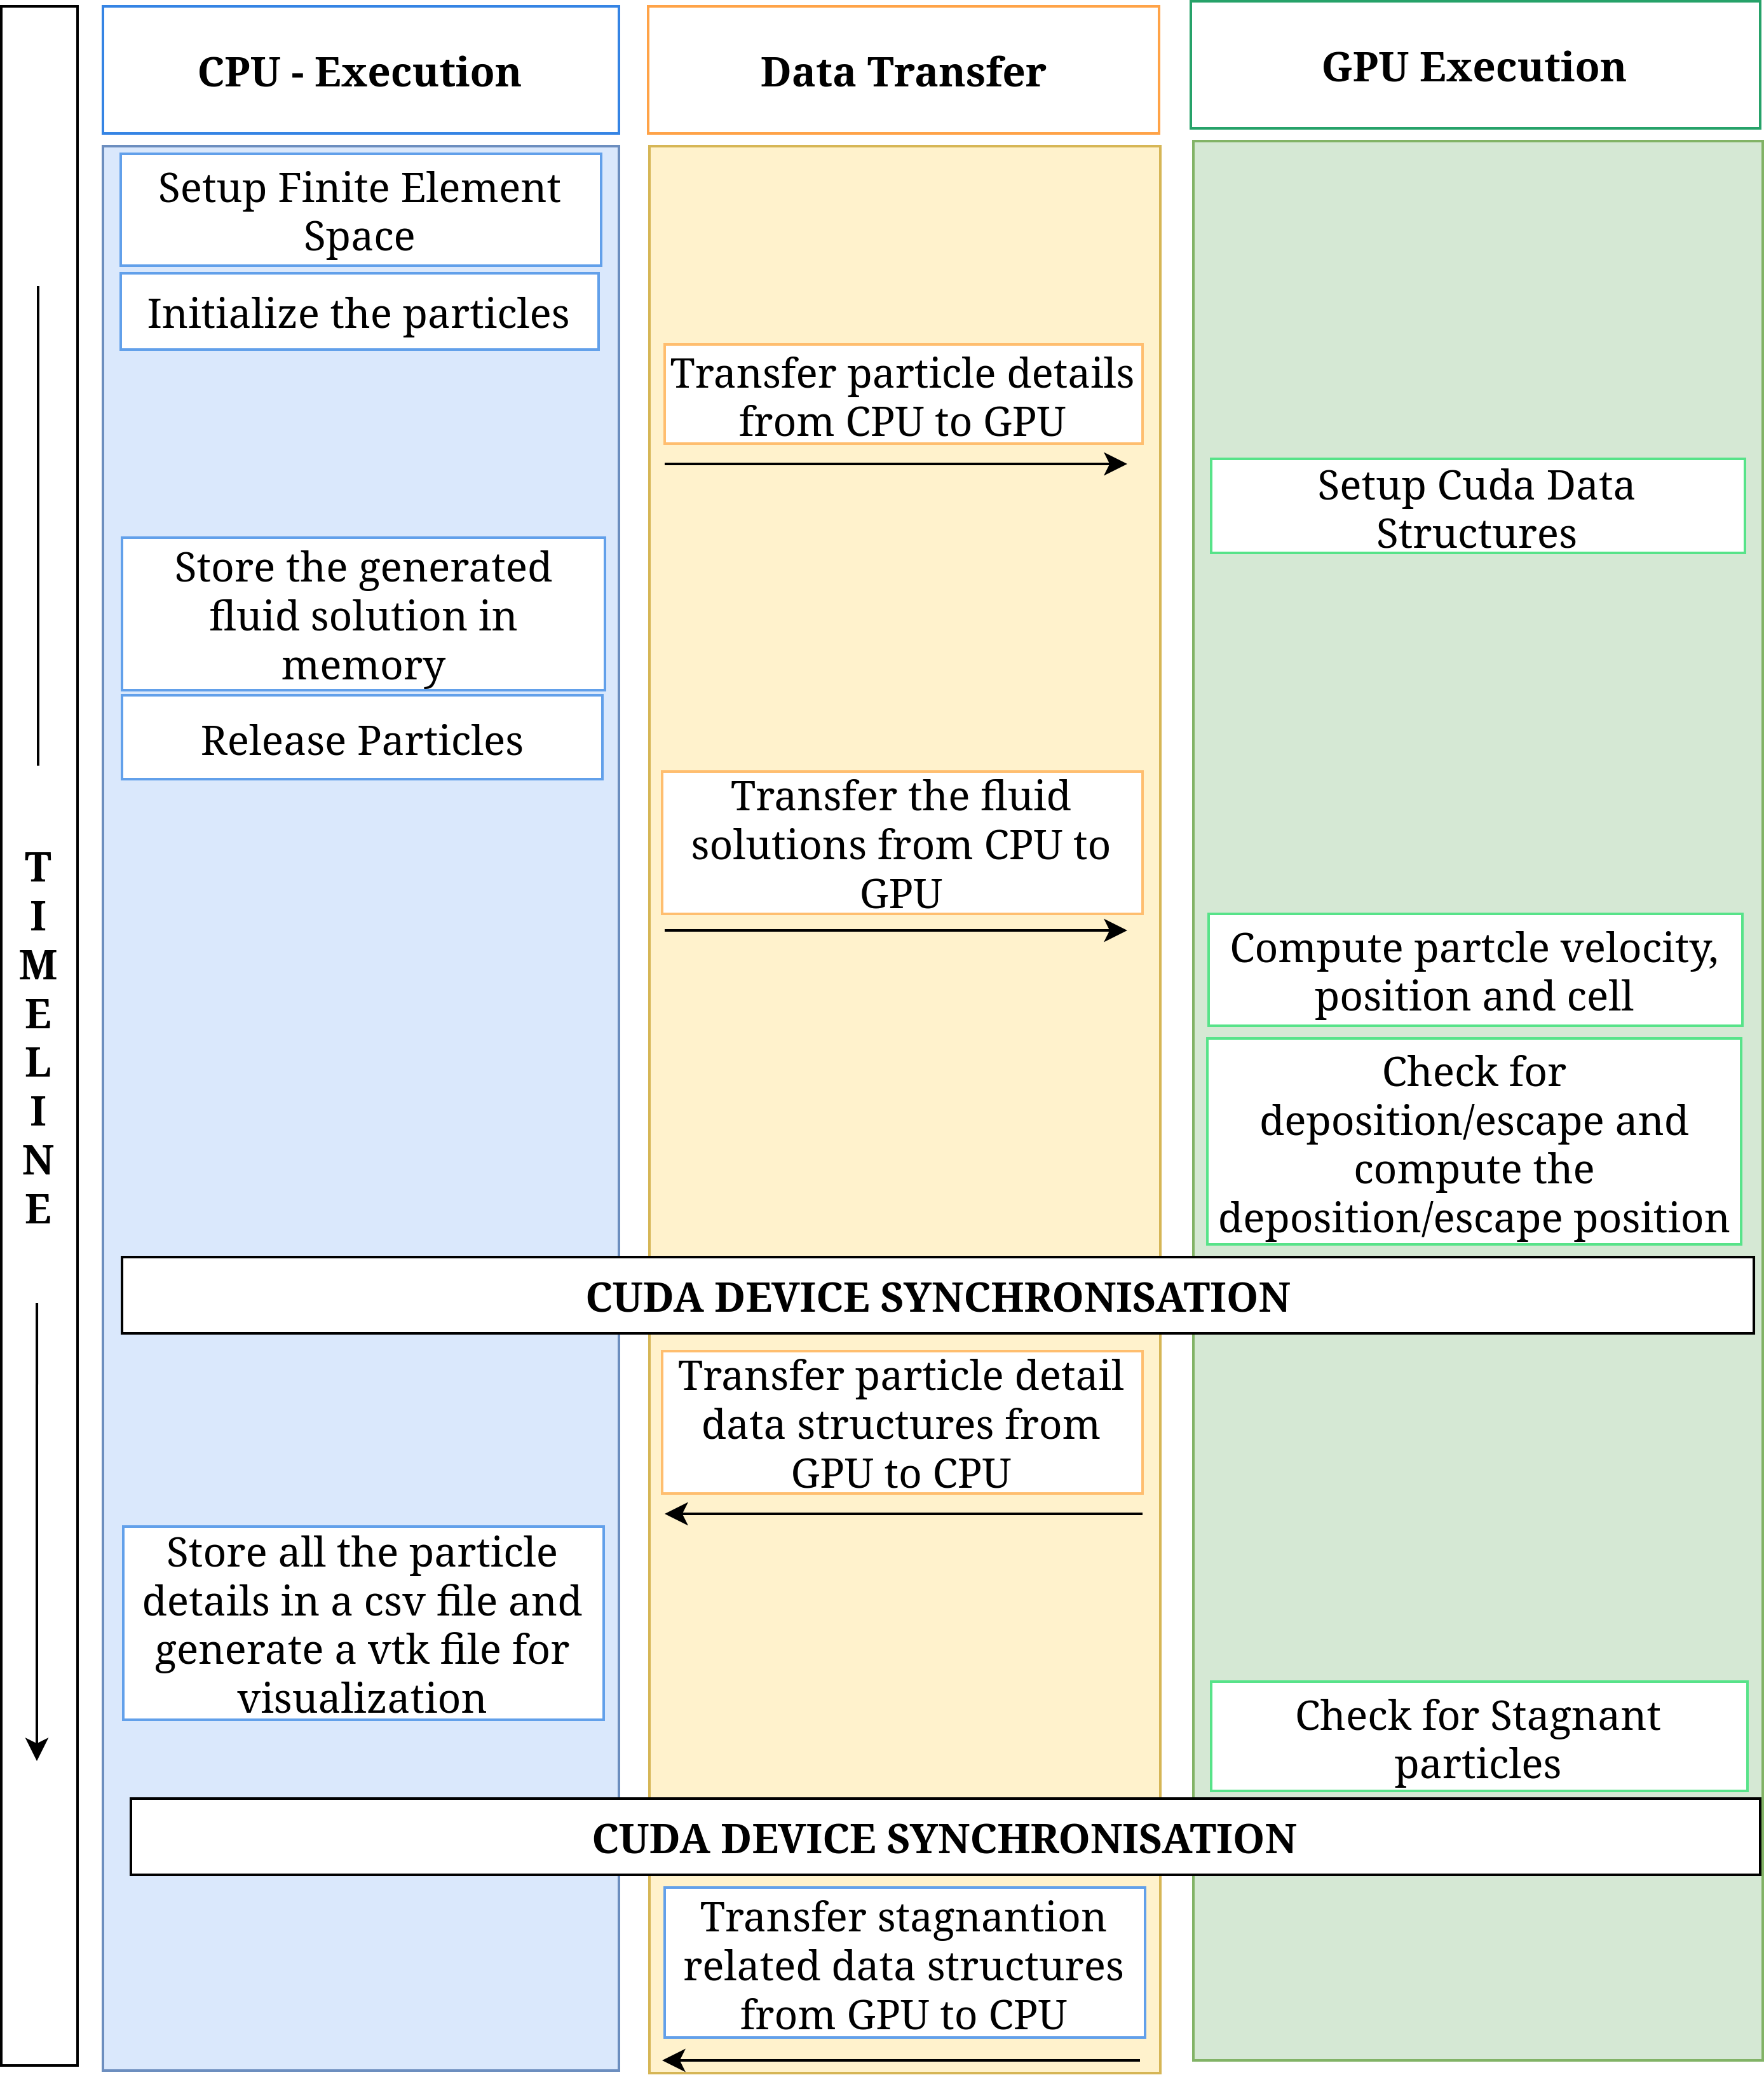
\includegraphics[width=.5\linewidth]{timeline}
\end{center}

\begin{itemize}
\item Mesh, Geometry (segmented), Begining of simulation, End of simulation
\end{itemize}
\vspace{0.1cm}
\begin{center}
  \vspace{-0.4cm}
  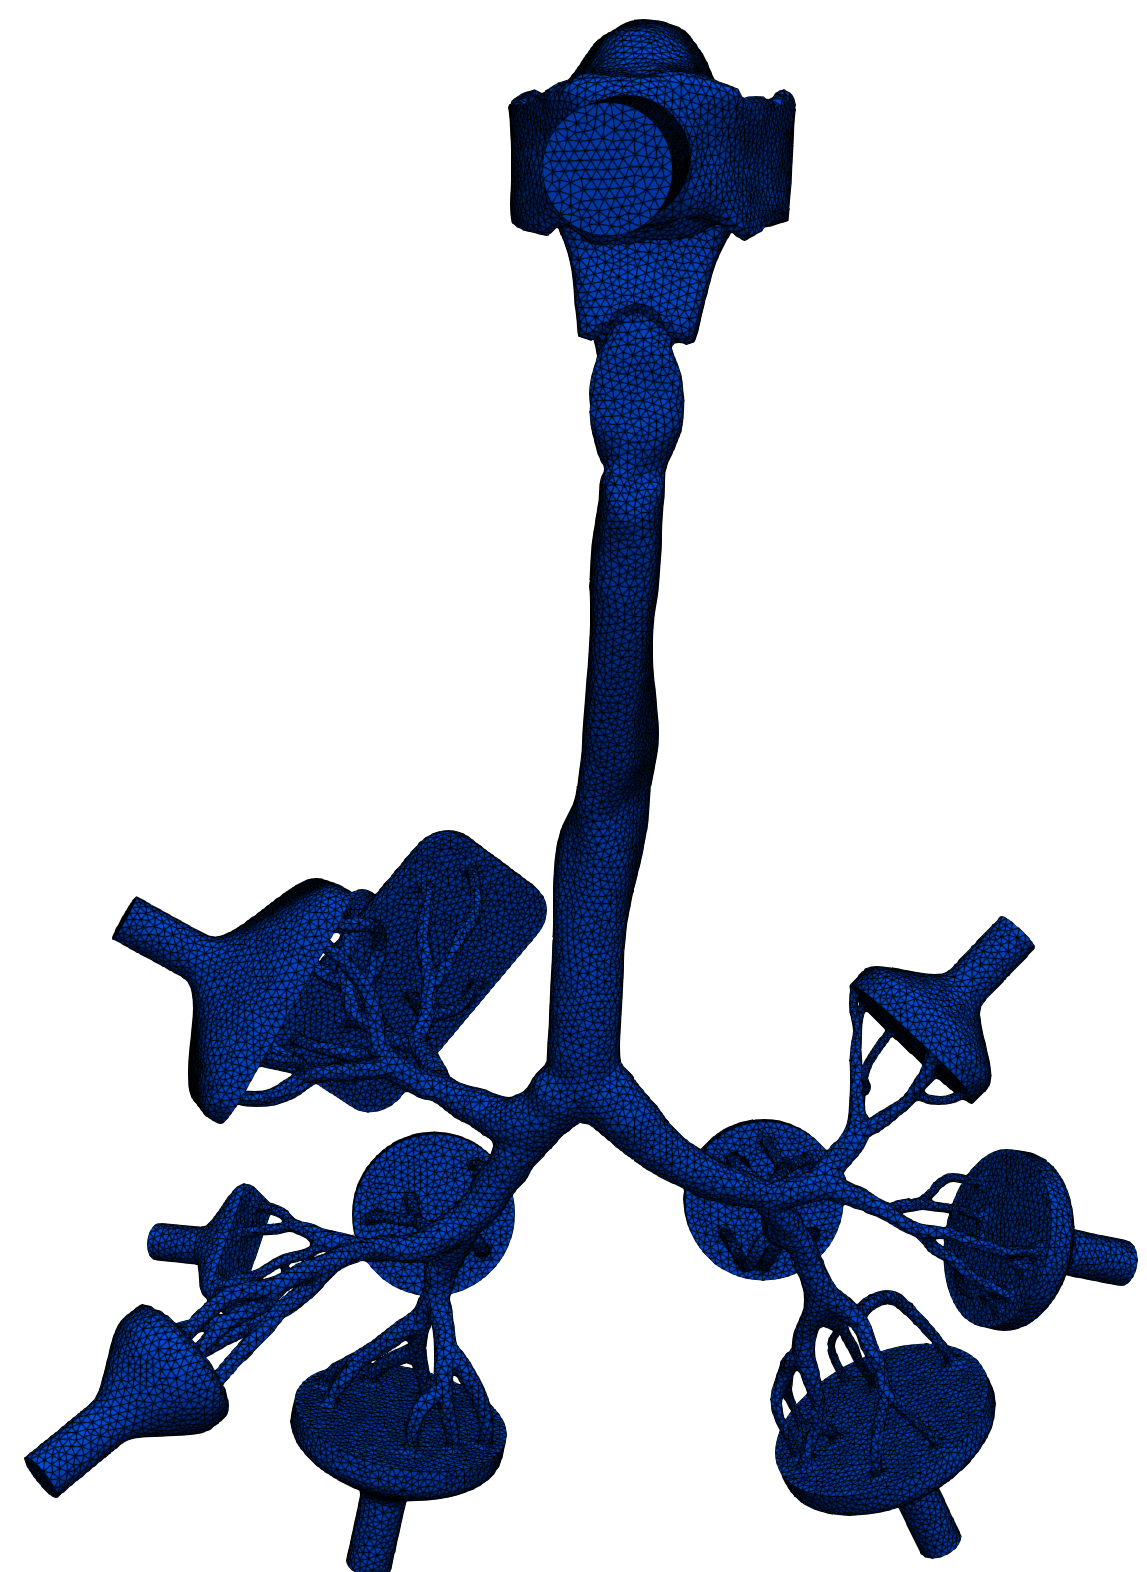
\includegraphics[width=.2\linewidth]{mesh}%
  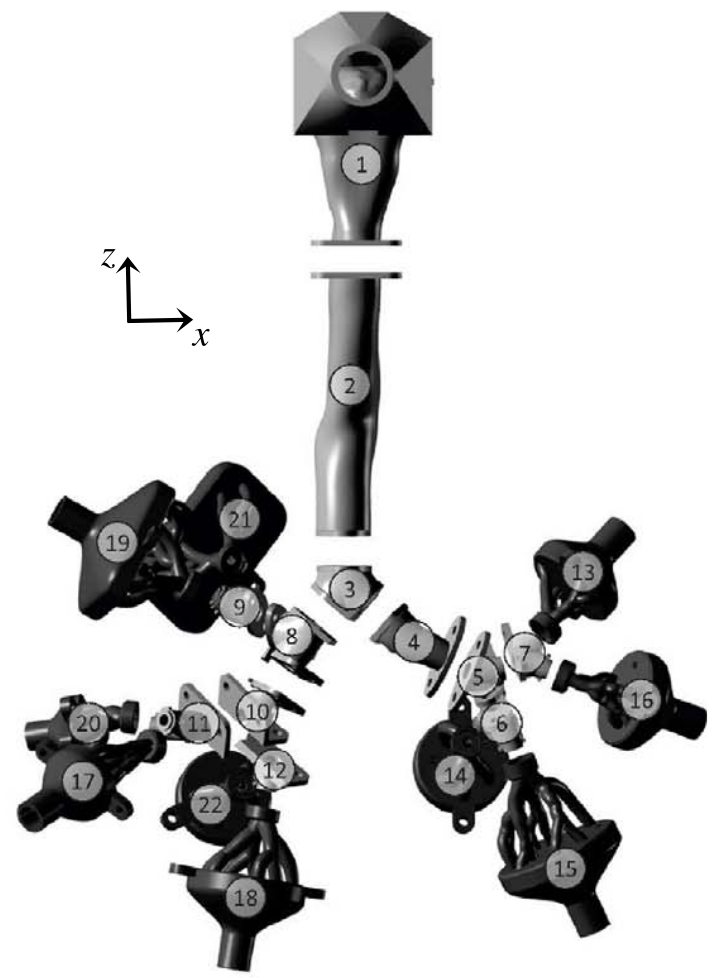
\includegraphics[width=.2\linewidth]{segments}\hspace{0.2cm}
  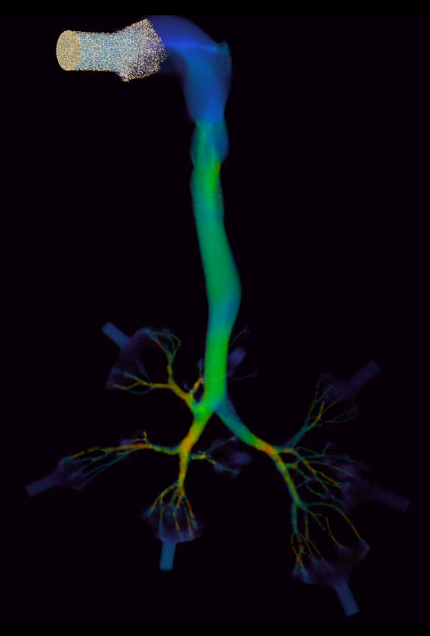
\includegraphics[width=.2\linewidth]{simulation_beg}%
  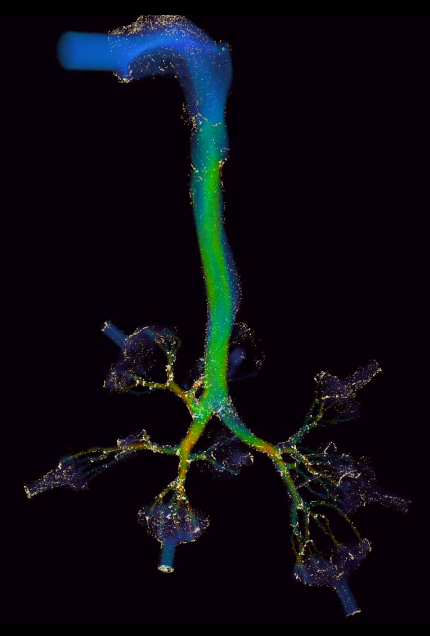
\includegraphics[width=.2\linewidth]{simulation_end}
\end{center}
% \vspace{0.25em}

% \vspace{0.3cm}
% \begin{center}
%   \vspace{-0.4cm}
%   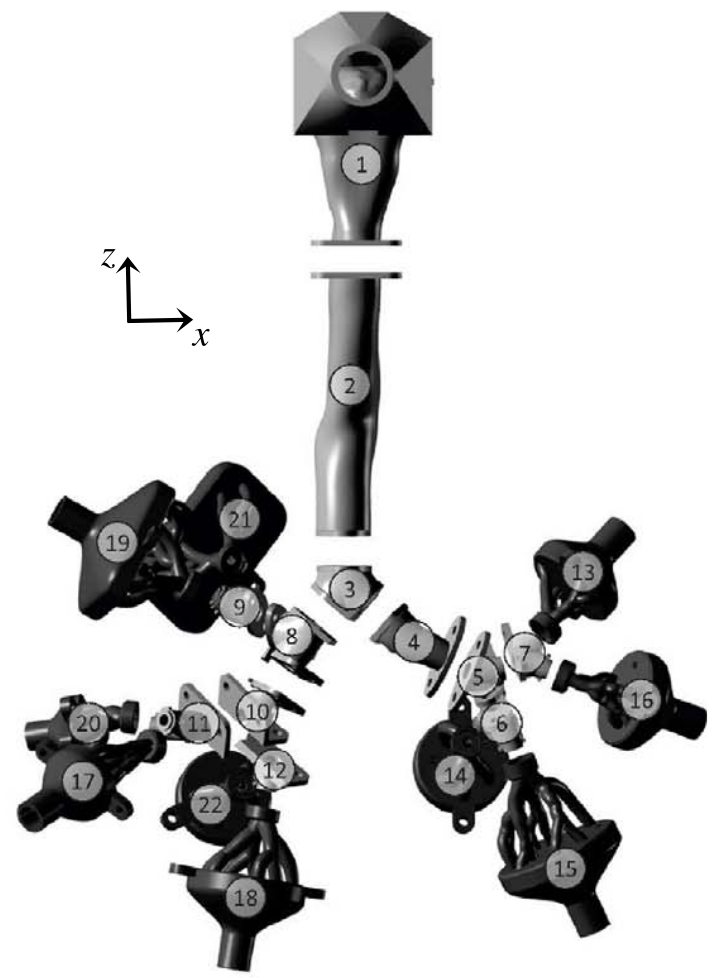
\includegraphics[width=.4\linewidth]{segments}%
%   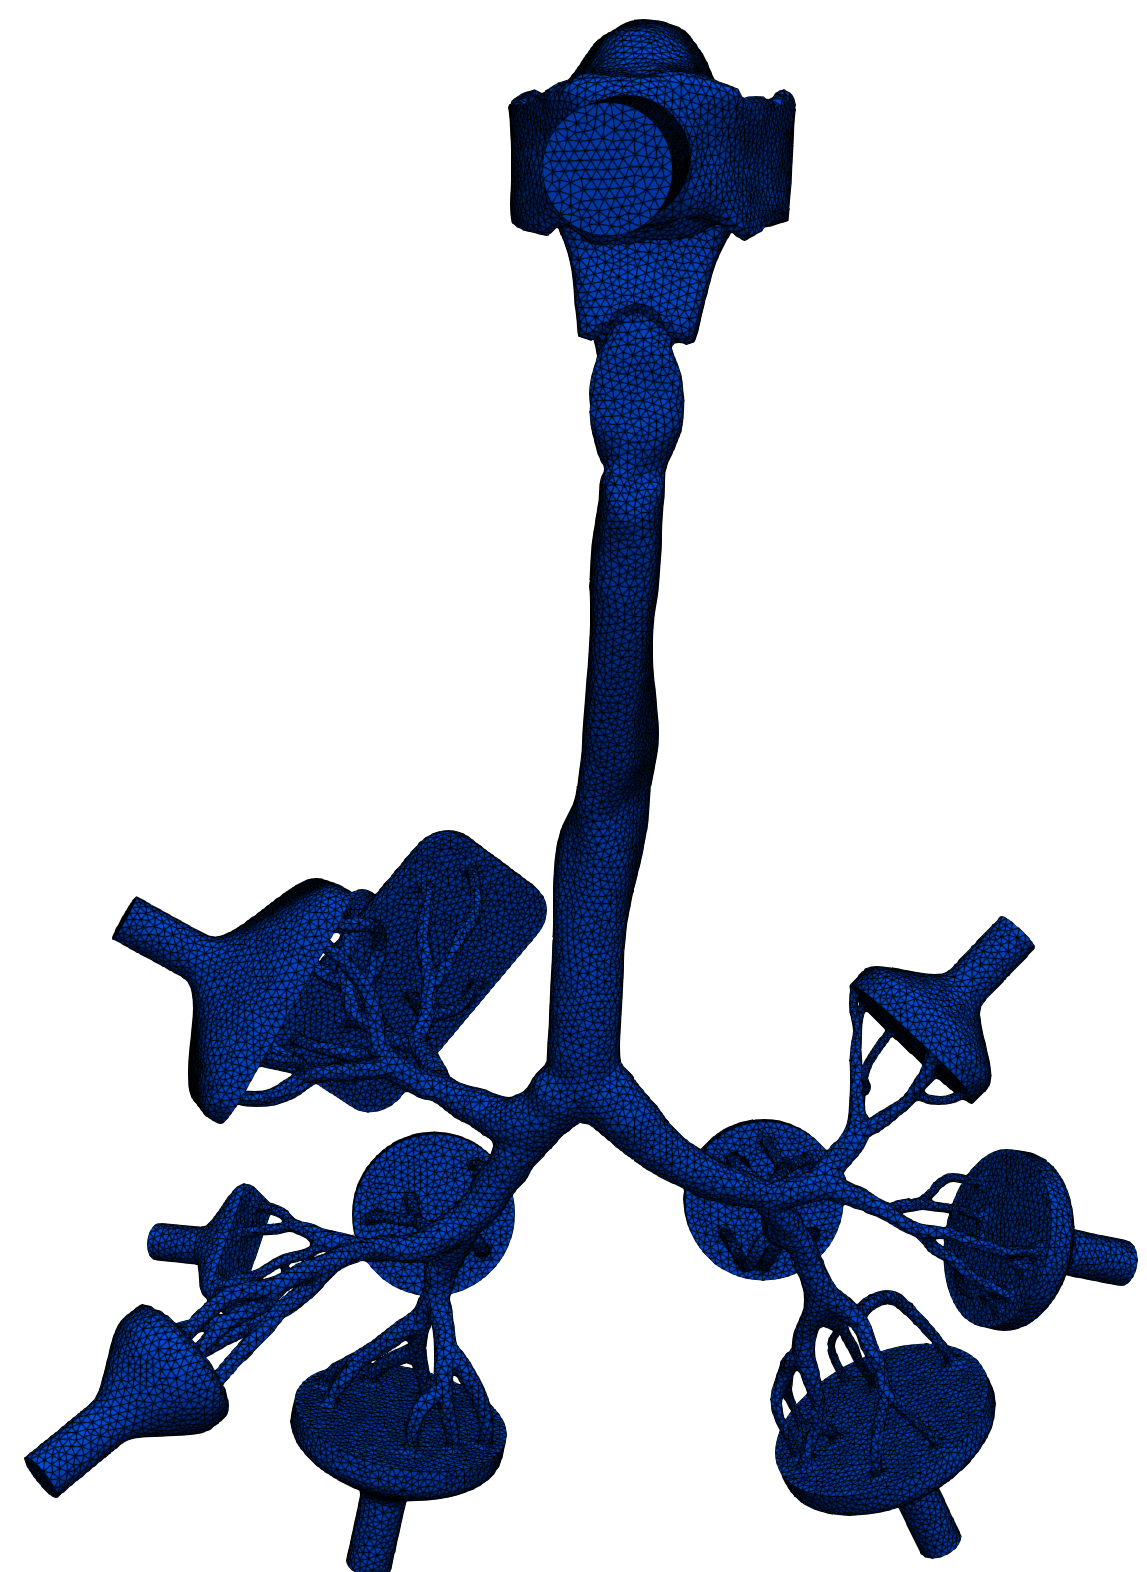
\includegraphics[width=.4\linewidth]{mesh}
% \end{center}
% \vspace{0.25em}
% \textbf{Computational Mesh:}

% \begin{tabular}{@{$\bullet$ }ll}
% Number of Vertices  &: 65,725 \\
% Number of Cells     &: 276,577   \\
% Number of Boundary faces &: 590,950 \\
% DOF velocity fluid: &: 1,337,640 \\
% DOF velocity pressure &: 65,725 \\
% \end{tabular}

\vspace{2em} % Fill in to put references at the bottom
}

%%%%%%%%%%%%%%%%%%%%%%%%%%%%%%%%%%%%%%%%%%%%%%%%%%%%%%%%%%%%%%%%%%%%%%%%%%%%%%
  \headerbox{\mytitlefont Results}{name=goal,column=1,row=0,span=1, below=description }{
%%%%%%%%%%%%%%%%%%%%%%%%%%%%%%%%%%%%%%%%%%%%%%%%%%%%%%%%%%%%%%%%%%%%%%%%%%%%%%
  \mytextfont
  % Put some results here

\begin{itemize}
\item We validated the results of our model with existing literature\textsuperscript{[2]} using deposition fraction at different segments of the lungs (8$\mu$m on left and 10$\mu$m on right).
\end{itemize}

\vspace{0.3cm}
\begin{center}
  \vspace{-0.4cm}
  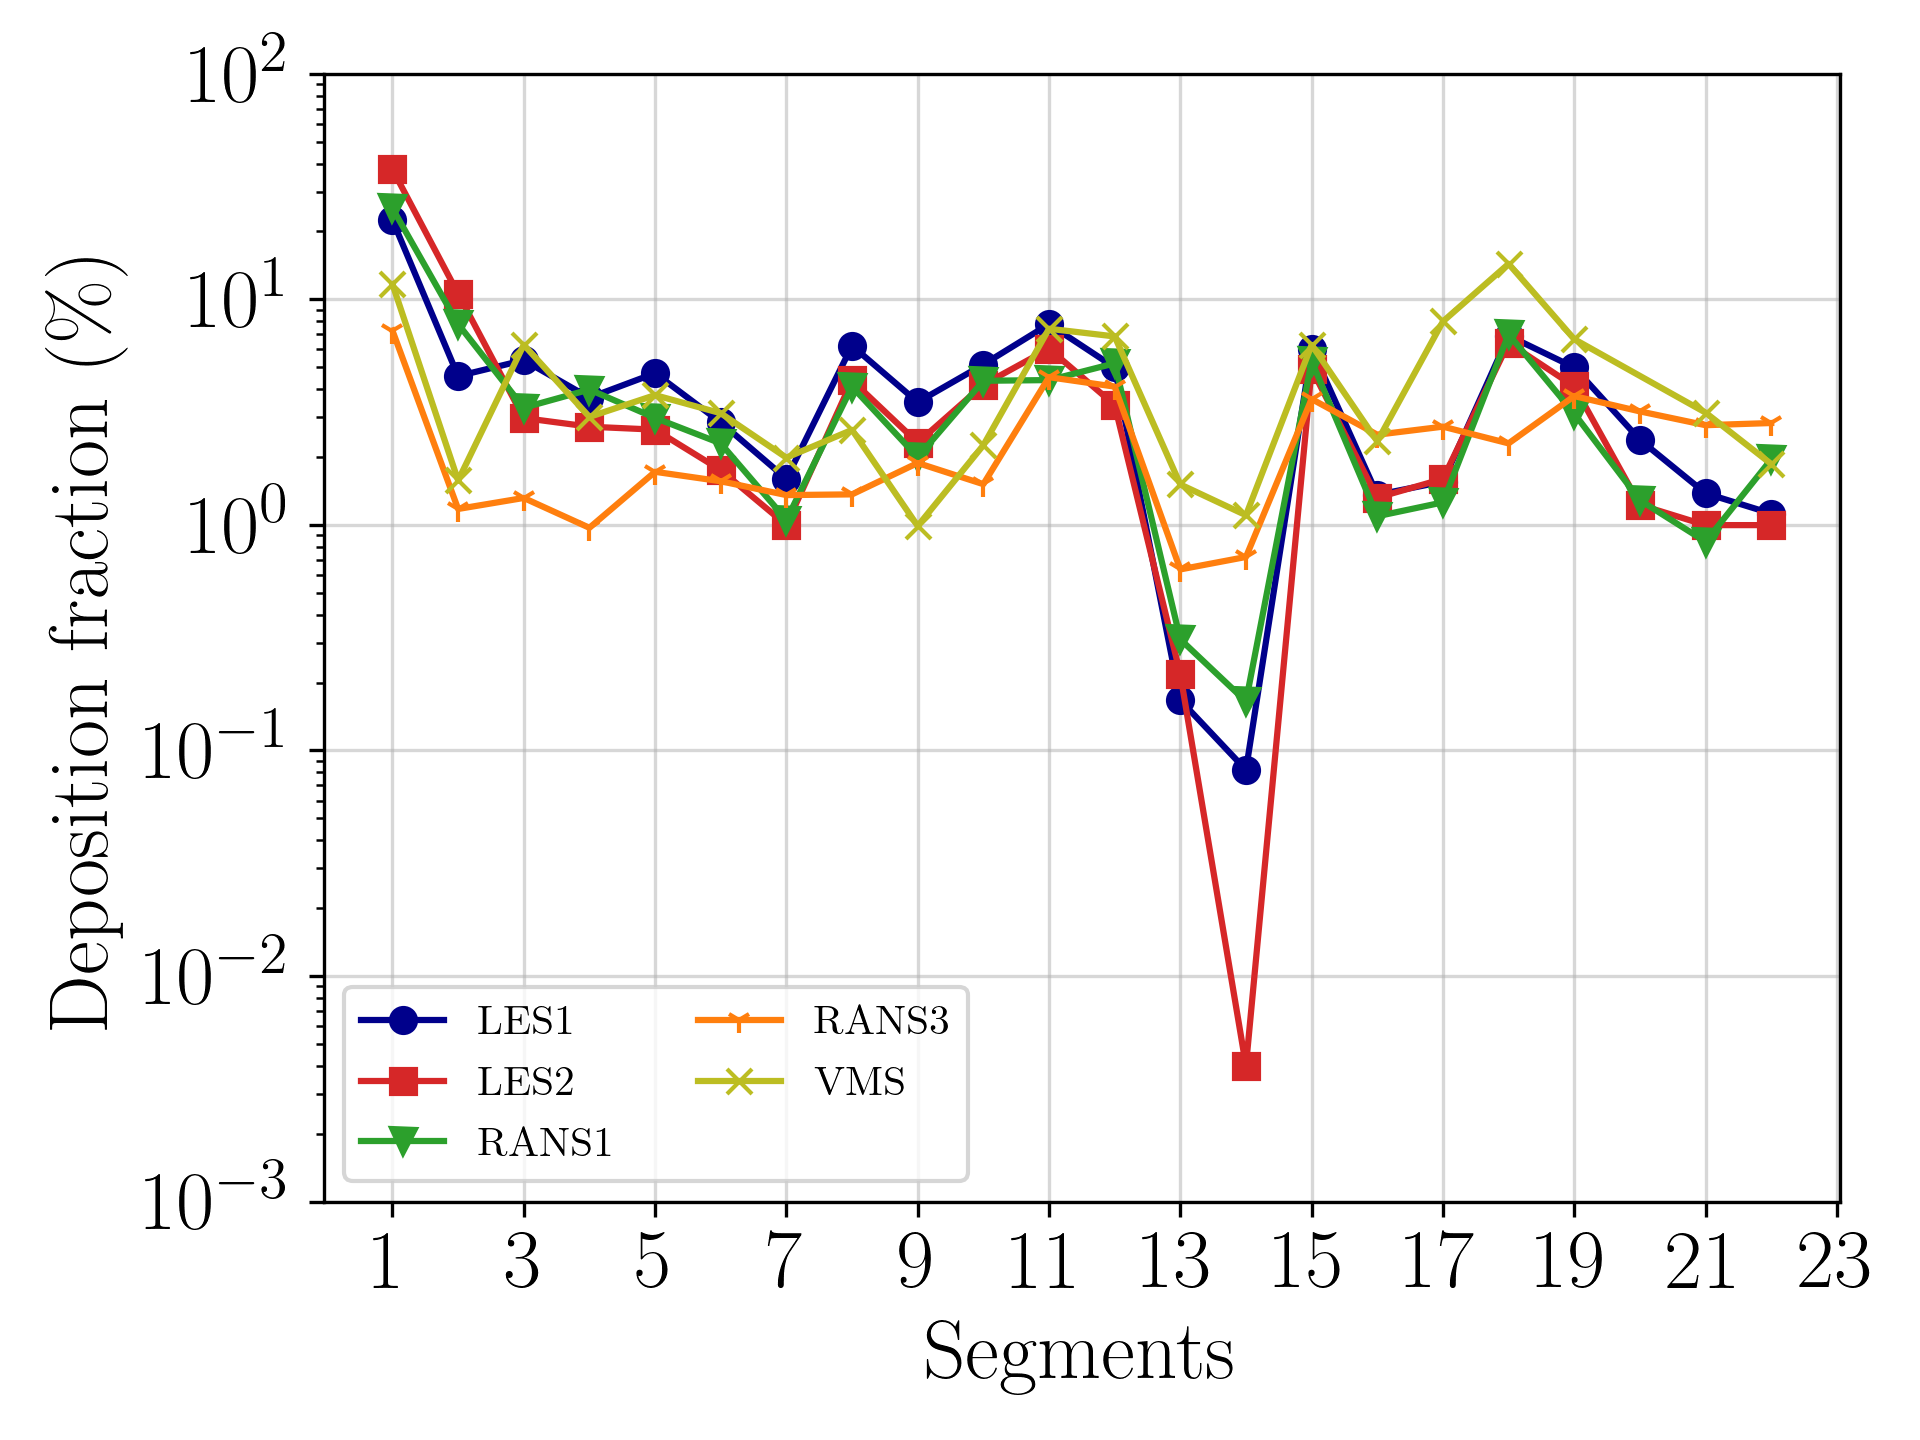
\includegraphics[width=.5\linewidth]{df8}%
  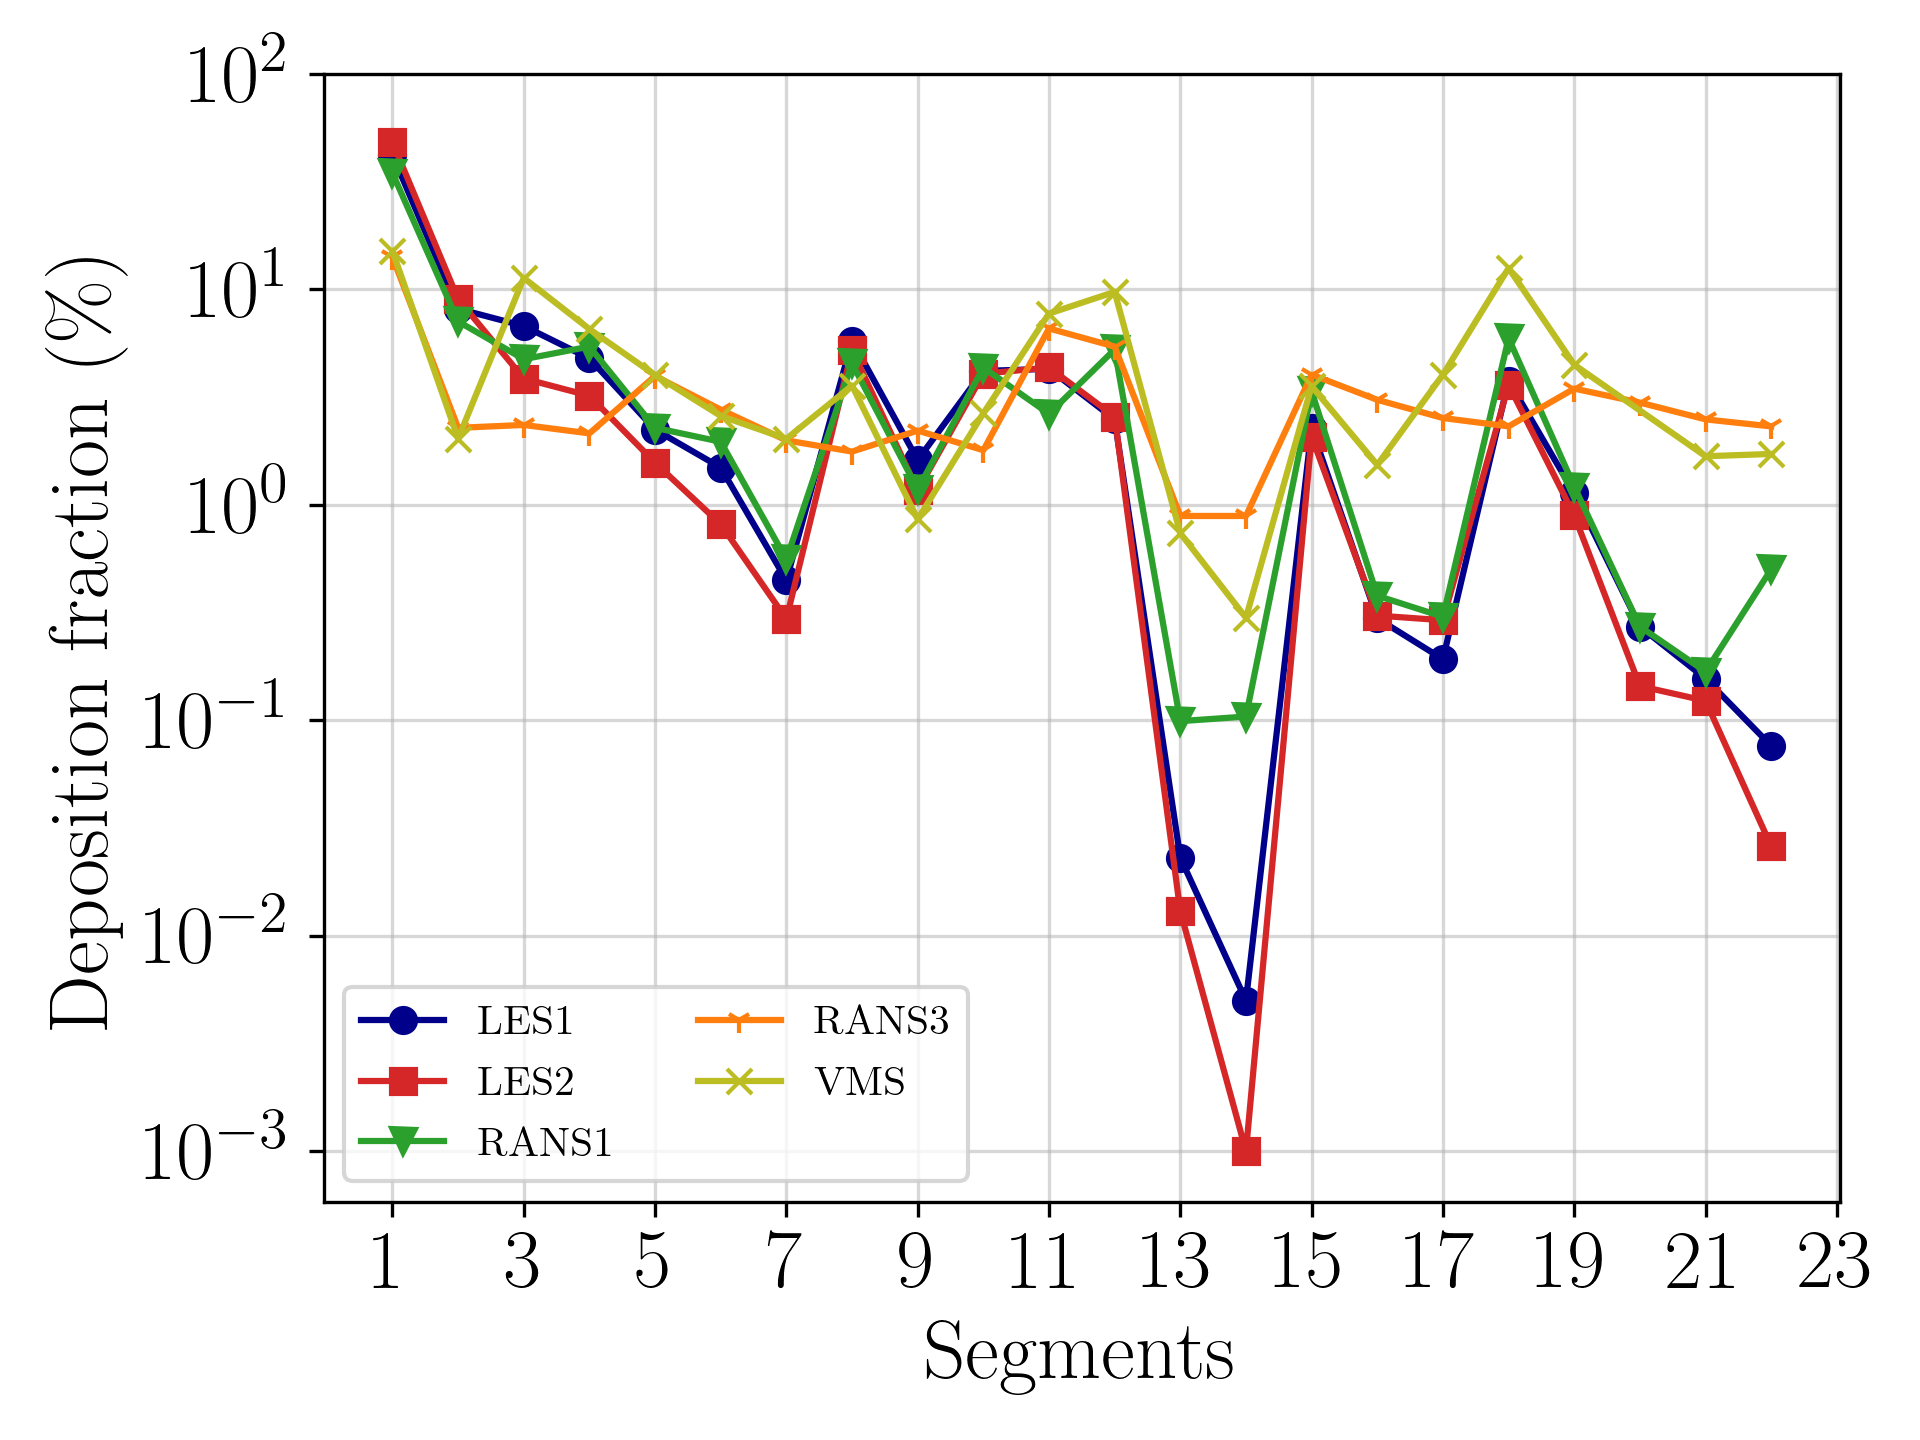
\includegraphics[width=.5\linewidth]{df10}
\end{center}
\vspace{0.25em}

\begin{itemize}
\item We achieved speedups of 13x for OpenMP and 220x for GPU when compared to the sequential.
\end{itemize}

\vspace{0.3cm}
\begin{center}
  \vspace{-0.4cm}
  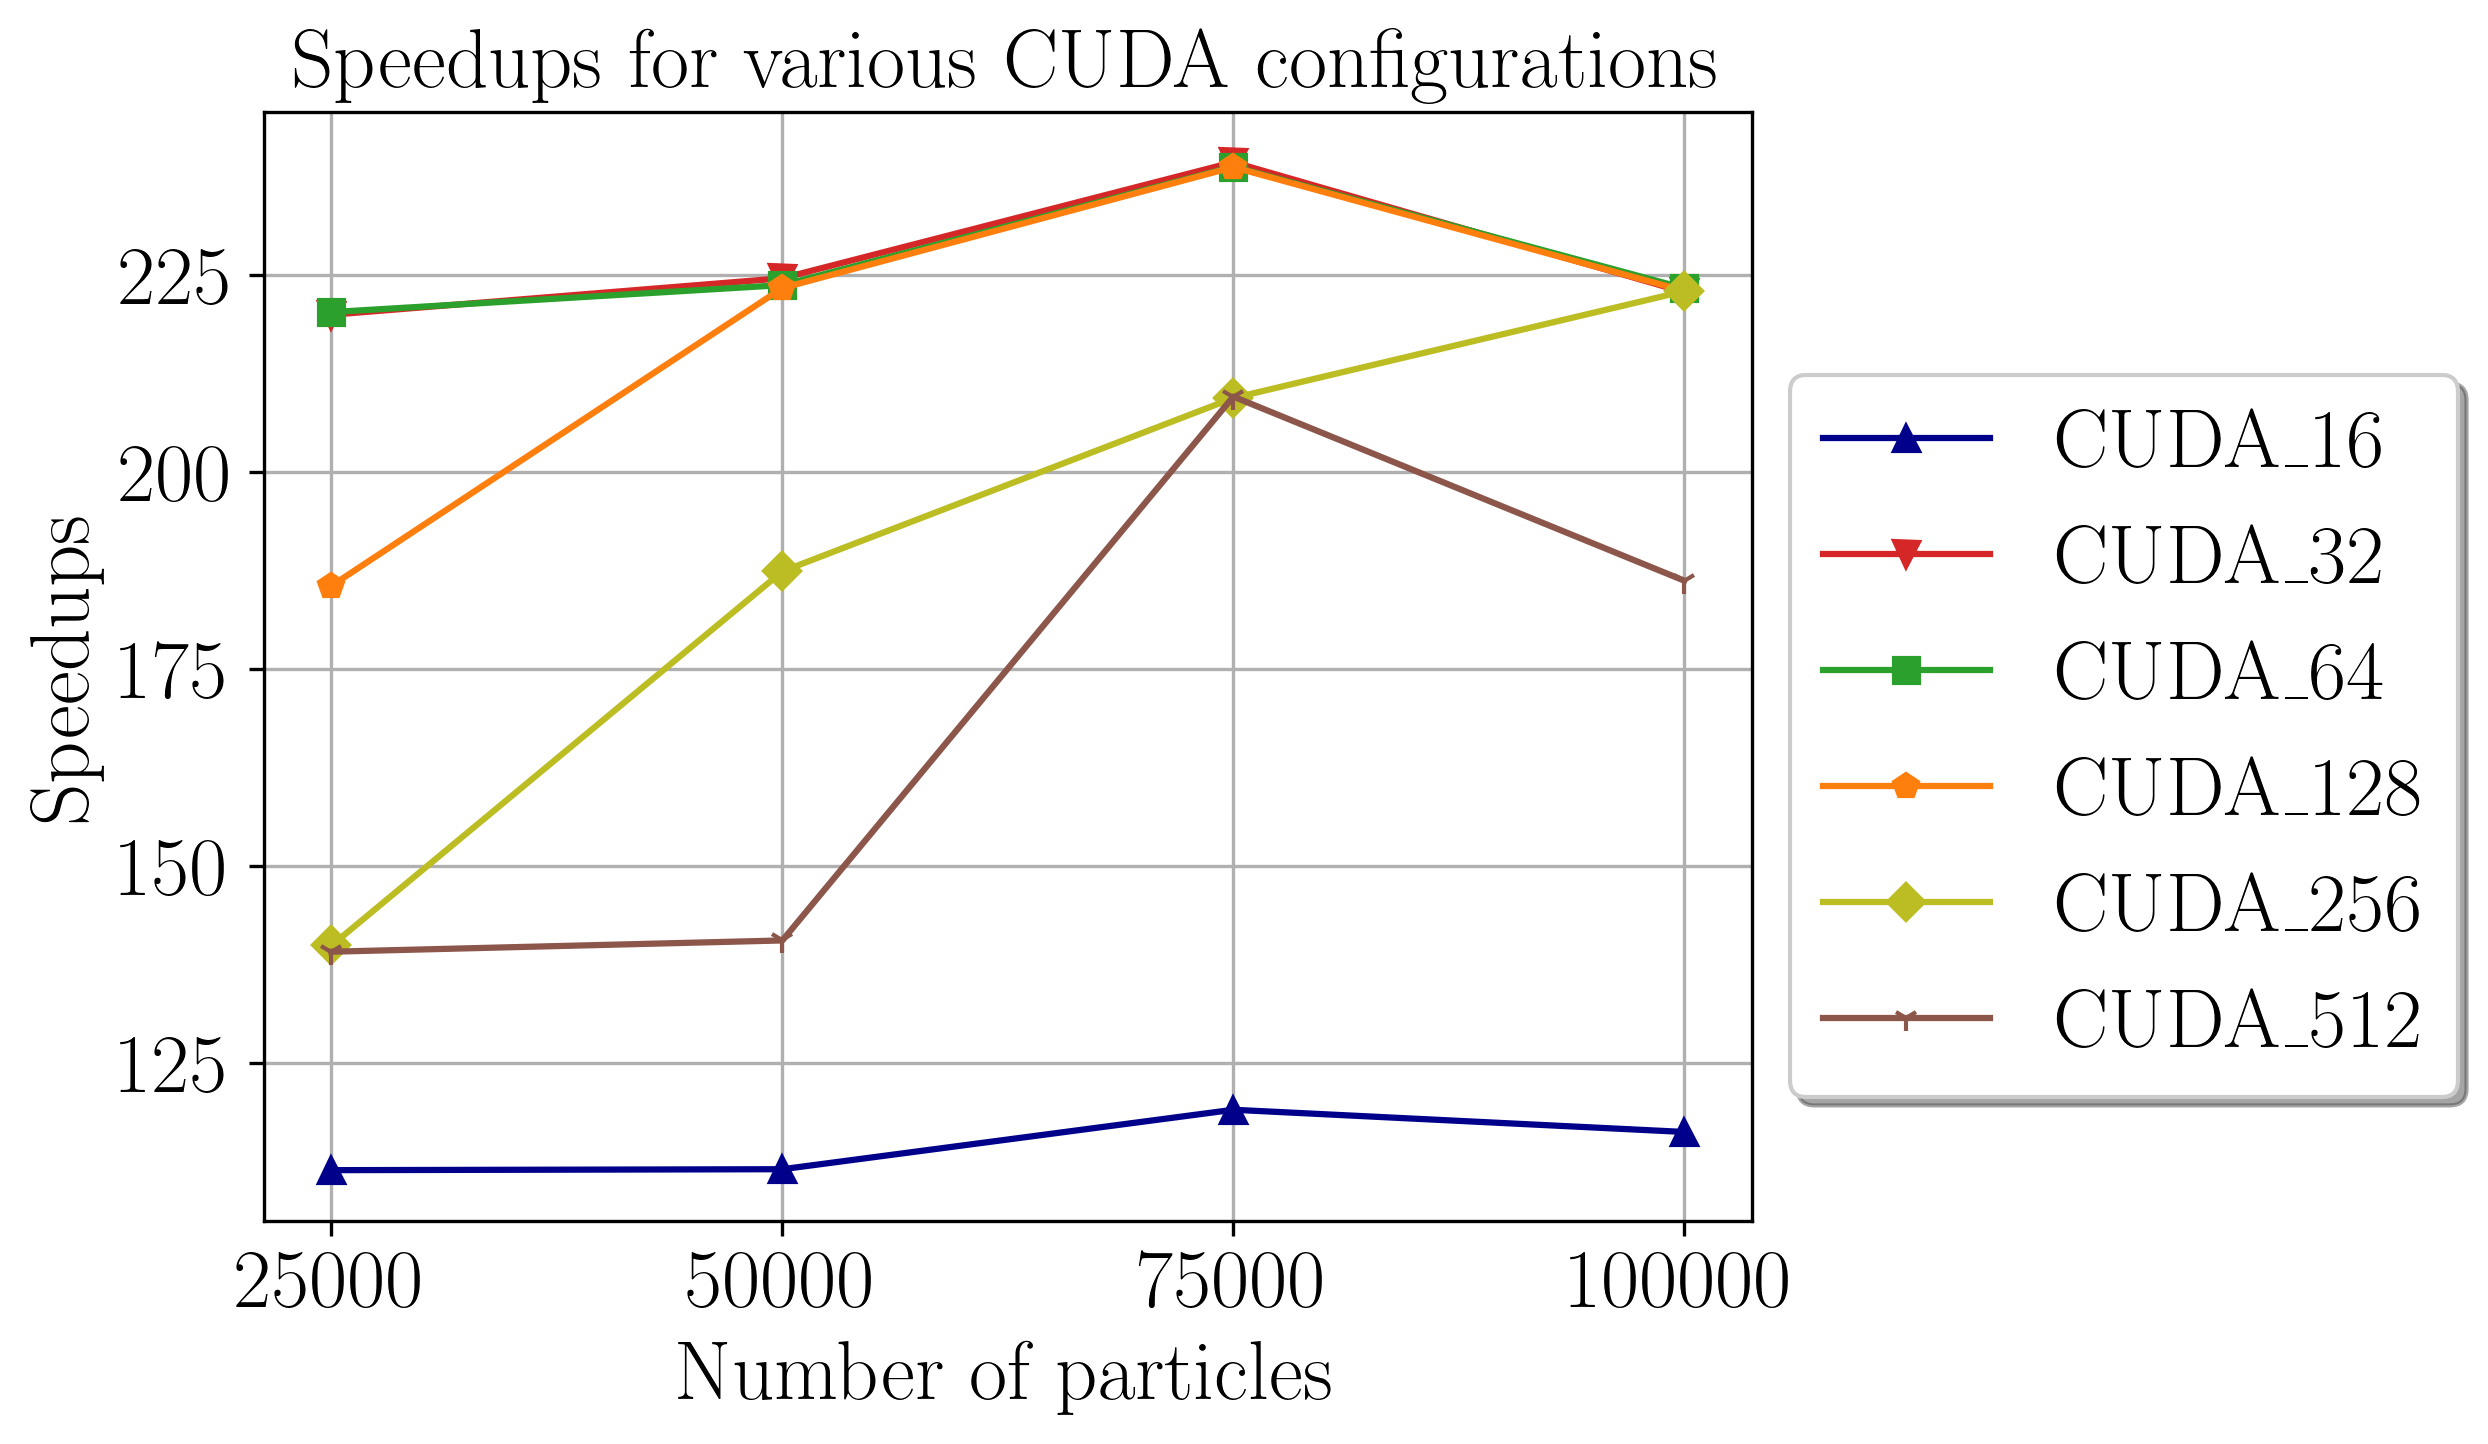
\includegraphics[width=.5\linewidth]{speedup}%
  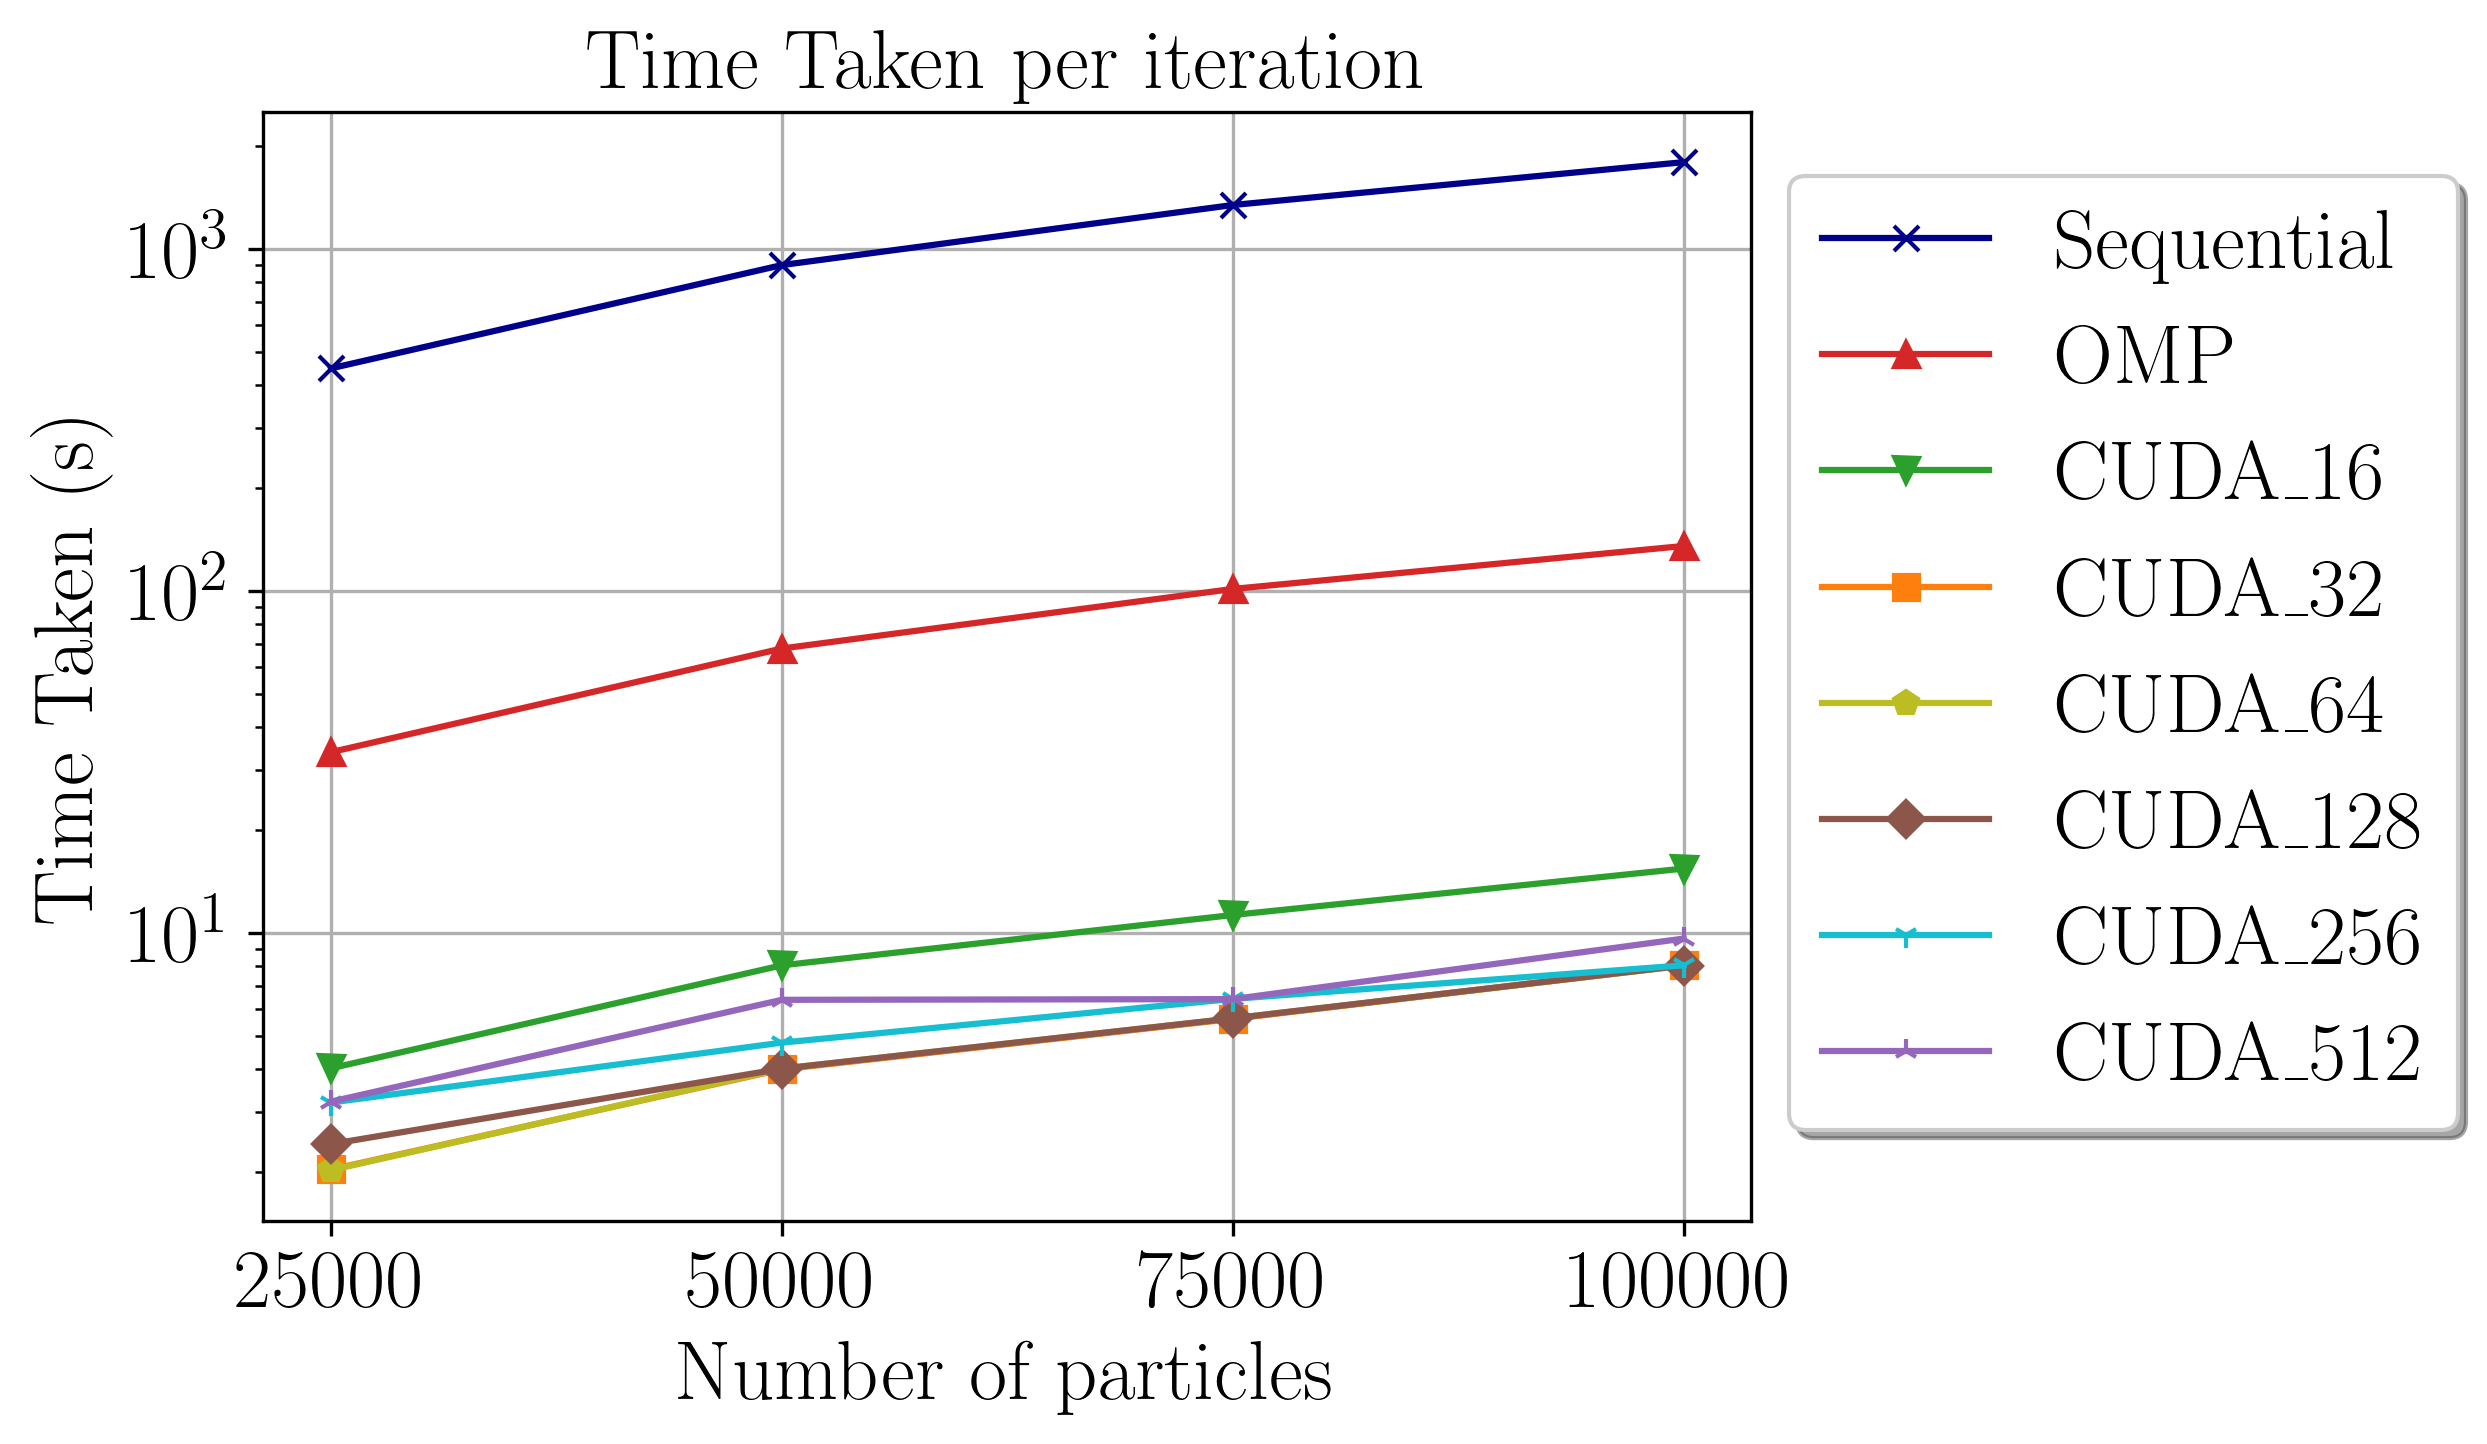
\includegraphics[width=.5\linewidth]{time}
\end{center}
\vspace{0.25em}

}

%%%%%%%%%%%%%%%%%%%%%%%%%%%%%%%%%%%%%%%%%%%%%%%%%%%%%%%%%%%%%%%%%%%%%%%%%%%%%%
  \headerbox{\mytitlefont Future Plan}{name=future,column=1,row=0,span=1, below=goal }{
%%%%%%%%%%%%%%%%%%%%%%%%%%%%%%%%%%%%%%%%%%%%%%%%%%%%%%%%%%%%%%%%%%%%%%%%%%%%%%
	\mytextfont
  \begin{itemize}
\item Integrate CUDA with MPI on a distributed computing setup to further improve the scalability of the particle tracking.
\item Implement asynchronous data transfer within the GPU using CUDA streams to overlap the data-transfer with computation.
\end{itemize}

}

%%%%%%%%%%%%%%%%%%%%%%%%%%%%%%%%%%%%%%%%%%%%%%%%%%%%%%%%%%%%%%%%%%%%%%%%%%%%%%
  \headerbox{References}{headerColorOne=wasp_banner_grey, borderColor=wasp_banner_grey, name=results,column=1,row=0,span=1, below=future }{
%%%%%%%%%%%%%%%%%%%%%%%%%%%%%%%%%%%%%%%%%%%%%%%%%%%%%%%%%%%%%%%%%%%%%%%%%%%%%%
	\mytextfont
  \small
\vspace{-0.5cm}
\fcolorbox{white}{white}{\hspace{-0.5cm}\parbox{0.1\linewidth}{\centering [1]}\parbox{0.7\linewidth}{\footnotesize\smaller ParMooN -- a modernized program package based on mapped finite elements\\\tiny U. Wilbrandt, C. Bartsch, N. Ahmed, N. Alia, F. Anker, L. Blank, A. Caiazzo, S. Ganesan, S. Giere, G. Matthies, R. Meesala, A. Shamim, J. Venkatesan, and V. John\\Computers \& Mathematics with Applications, 2017}}

\fcolorbox{white}{white}{\hspace{-0.5cm}\parbox{0.1\linewidth}{\centering [2]}\parbox{0.7\linewidth}{\footnotesize\smaller Regional aerosol deposition in the human airways: The SimInhale benchmark case and a critical assessment of in silico methods.\\\tiny P. Koullapis, S.C. Kassinos, J. Muela, C. Perez-Segarra, J. Rigola, O. Lehmkuhl, Y. Cui, M. Sommerfeld, J. Elcner, M. Jicha, I. Saveljic, N. Filipovic, F. Lizal, and L. Nicolaou\\European Journal of Pharmaceutical Sciences, 2018}}

% \vspace{-0.5cm}
% \fcolorbox{white}{white}{\hspace{-0.5cm}\parbox{0.1\linewidth}{\centering [1]}\parbox{1.3cm}{\includegraphics[trim=28mm 10mm 35mm 15mm,clip,width=0.8cm]{qracm}}\parbox{0.7\linewidth}{\footnotesize\smaller Five Challenges in Cloud-Enabled Intelligence and Control\\\tiny T. Abdelzaher, Y. Hao, K. Jayarajah, A. Misra, S. Yao, P. Skarin, D. Weerakoon and K. {\AA}rz{\'e}n\\ACM Transactions on Internet Technology, 2019}}\par\vspace{-0.4cm}
	
% \fcolorbox{white}{white}{\hspace{-0.5cm}\parbox{0.1\linewidth}{\centering [2]}\parbox{1.3cm}{\includegraphics[trim=25mm 10mm 35mm 10mm,clip,width=0.8cm]{qredge1}}\parbox{0.7\linewidth}{\footnotesize\smaller Towards Mission-Critical Control at the Edge and Over 5G\\\tiny Per Skarin, William Tärneberg, Karl-Erik Årzén, Maria Kihl\\Best paper award, IEEE Services (EDGE), 2-7 July, 2018, San Fran., CA, USA}}\par\vspace{-0.25cm}
	
% \fcolorbox{white}{white}{\hspace{-0.5cm}\parbox{0.1\linewidth}{\centering [5]}\parbox{1.3cm}{\includegraphics[trim=28mm 35mm 35mm 35mm,clip,width=0.8cm]{qrifac}}\parbox{0.7\linewidth}{\footnotesize\smaller Cloud-based model predictive control with variable horizon\\\tiny Per Skarin, Johan Eker, Karl-Erik Årzén\\Subm. to 21st World Congress of the International Federation of Automatic Control, 2020}}\par\vspace{-0.3cm}
}

\headerbox{}{name=foottext, column=0, span=2, above=bottom, textborder=none,headerborder=none,boxheaderheight=0pt,boxColorOne=wasp_banner_grey}{\hfill 
\includegraphics[height=1cm]{stars_transparent}}


\end{poster}
\end{document}

%%% Local Variables:
%%% mode: latex
%%% TeX-master: t
%%% End:
